\section{moeo\-Easy\-EA$<$ MOEOT $>$ Class Template Reference}
\label{classmoeoEasyEA}\index{moeoEasyEA@{moeoEasyEA}}
An easy class to design multi-objective evolutionary algorithms.  


{\tt \#include $<$moeo\-Easy\-EA.h$>$}

Inheritance diagram for moeo\-Easy\-EA$<$ MOEOT $>$::\begin{figure}[H]
\begin{center}
\leavevmode
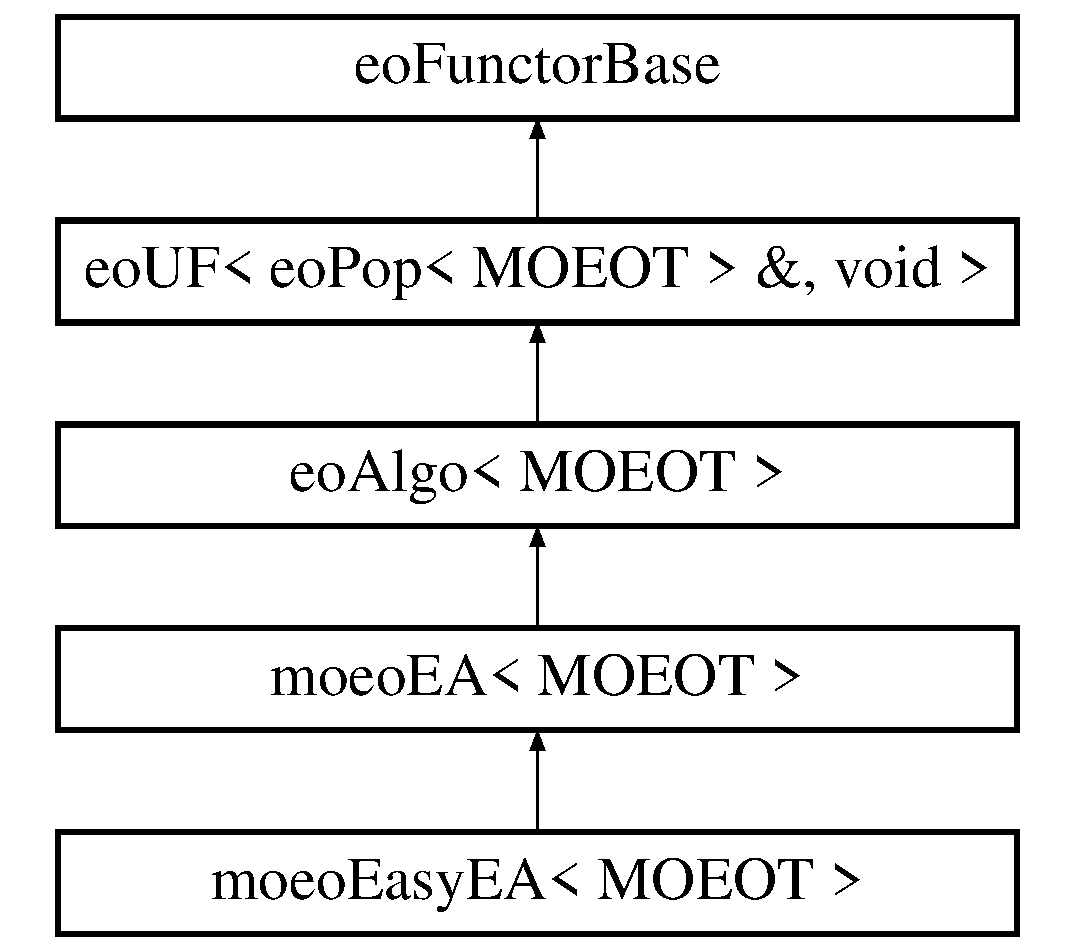
\includegraphics[height=5cm]{classmoeoEasyEA}
\end{center}
\end{figure}
\subsection*{Public Member Functions}
\begin{CompactItemize}
\item 
{\bf moeo\-Easy\-EA} ({\bf eo\-Continue}$<$ MOEOT $>$ \&\_\-continuator, {\bf eo\-Eval\-Func}$<$ MOEOT $>$ \&\_\-eval, {\bf eo\-Breed}$<$ MOEOT $>$ \&\_\-breed, {\bf eo\-Replacement}$<$ MOEOT $>$ \&\_\-replace, {\bf moeo\-Fitness\-Assignment}$<$ MOEOT $>$ \&\_\-fitness\-Eval, {\bf moeo\-Diversity\-Assignment}$<$ MOEOT $>$ \&\_\-diversity\-Eval, bool \_\-eval\-Fit\-And\-Div\-Before\-Selection=false)
\begin{CompactList}\small\item\em Ctor. \item\end{CompactList}\item 
virtual void {\bf operator()} ({\bf eo\-Pop}$<$ MOEOT $>$ \&\_\-pop)
\begin{CompactList}\small\item\em Applies a few generation of evolution to the population \_\-pop. \item\end{CompactList}\end{CompactItemize}
\subsection*{Protected Attributes}
\begin{CompactItemize}
\item 
{\bf eo\-Continue}$<$ MOEOT $>$ \& {\bf continuator}\label{classmoeoEasyEA_5f5b76acbaf99a6a3ee2710da07dde29}

\begin{CompactList}\small\item\em the stopping criteria \item\end{CompactList}\item 
{\bf eo\-Eval\-Func}$<$ MOEOT $>$ \& {\bf eval}\label{classmoeoEasyEA_26e8ebce6a1bc3216e20171688ba6b83}

\begin{CompactList}\small\item\em the evaluation functions \item\end{CompactList}\item 
{\bf eo\-Pop\-Loop\-Eval}$<$ MOEOT $>$ {\bf loop\-Eval}\label{classmoeoEasyEA_c1d492090805bf322c07159a9238a7ae}

\begin{CompactList}\small\item\em to evaluate the whole population \item\end{CompactList}\item 
{\bf eo\-Pop\-Eval\-Func}$<$ MOEOT $>$ \& {\bf pop\-Eval}\label{classmoeoEasyEA_189a8f5196844907ff71f386d95bf415}

\begin{CompactList}\small\item\em to evaluate the whole population \item\end{CompactList}\item 
{\bf eo\-Breed}$<$ MOEOT $>$ \& {\bf breed}\label{classmoeoEasyEA_35d5909694019d1b0d52347c72a9092e}

\begin{CompactList}\small\item\em the breeder \item\end{CompactList}\item 
{\bf eo\-Replacement}$<$ MOEOT $>$ \& {\bf replace}\label{classmoeoEasyEA_1872664368d198f983d11a96f0ee3d8d}

\begin{CompactList}\small\item\em the replacment strategy \item\end{CompactList}\item 
{\bf moeo\-Fitness\-Assignment}$<$ MOEOT $>$ \& {\bf fitness\-Eval}\label{classmoeoEasyEA_1268fc2f0b62fe51bca17d4efb51954b}

\begin{CompactList}\small\item\em the fitness assignment strategy \item\end{CompactList}\item 
{\bf moeo\-Diversity\-Assignment}$<$ MOEOT $>$ \& {\bf diversity\-Eval}\label{classmoeoEasyEA_b9d1b3790072dbbbe0012a252bab95f4}

\begin{CompactList}\small\item\em the diversity assignment strategy \item\end{CompactList}\item 
bool {\bf eval\-Fit\-And\-Div\-Before\-Selection}\label{classmoeoEasyEA_856a19d9a7c180fe33ce7a5bb010edcc}

\begin{CompactList}\small\item\em if this parameter is set to 'true', the fitness and the diversity of the whole population will be re-evaluated before the selection process \item\end{CompactList}\end{CompactItemize}


\subsection{Detailed Description}
\subsubsection*{template$<$class MOEOT$>$ class moeo\-Easy\-EA$<$ MOEOT $>$}

An easy class to design multi-objective evolutionary algorithms. 



Definition at line 31 of file moeo\-Easy\-EA.h.

\subsection{Constructor \& Destructor Documentation}
\index{moeoEasyEA@{moeo\-Easy\-EA}!moeoEasyEA@{moeoEasyEA}}
\index{moeoEasyEA@{moeoEasyEA}!moeoEasyEA@{moeo\-Easy\-EA}}
\subsubsection{\setlength{\rightskip}{0pt plus 5cm}template$<$class MOEOT$>$ {\bf moeo\-Easy\-EA}$<$ MOEOT $>$::{\bf moeo\-Easy\-EA} ({\bf eo\-Continue}$<$ MOEOT $>$ \& {\em \_\-continuator}, {\bf eo\-Eval\-Func}$<$ MOEOT $>$ \& {\em \_\-eval}, {\bf eo\-Breed}$<$ MOEOT $>$ \& {\em \_\-breed}, {\bf eo\-Replacement}$<$ MOEOT $>$ \& {\em \_\-replace}, {\bf moeo\-Fitness\-Assignment}$<$ MOEOT $>$ \& {\em \_\-fitness\-Eval}, {\bf moeo\-Diversity\-Assignment}$<$ MOEOT $>$ \& {\em \_\-diversity\-Eval}, bool {\em \_\-eval\-Fit\-And\-Div\-Before\-Selection} = {\tt false})\hspace{0.3cm}{\tt  [inline]}}\label{classmoeoEasyEA_7fe81a5e24bd69d9f6de172d2bbe059a}


Ctor. 

\begin{Desc}
\item[Parameters:]
\begin{description}
\item[{\em \_\-continuator}]the stopping criteria \item[{\em \_\-eval}]the evaluation functions \item[{\em \_\-breed}]the breeder \item[{\em \_\-replace}]the replacment strategy \item[{\em \_\-fitness\-Eval}]the fitness evaluation scheme \item[{\em \_\-diversity\-Eval}]the diversity evaluation scheme \item[{\em \_\-eval\-Fit\-And\-Div\-Before\-Selection}]put this parameter to 'true' if you want to re-evalue the fitness and the diversity of the population before the selection process \end{description}
\end{Desc}


Definition at line 45 of file moeo\-Easy\-EA.h.

\subsection{Member Function Documentation}
\index{moeoEasyEA@{moeo\-Easy\-EA}!operator()@{operator()}}
\index{operator()@{operator()}!moeoEasyEA@{moeo\-Easy\-EA}}
\subsubsection{\setlength{\rightskip}{0pt plus 5cm}template$<$class MOEOT$>$ virtual void {\bf moeo\-Easy\-EA}$<$ MOEOT $>$::operator() ({\bf eo\-Pop}$<$ MOEOT $>$ \& {\em \_\-pop})\hspace{0.3cm}{\tt  [inline, virtual]}}\label{classmoeoEasyEA_f18e8fd179fbb2b89f4a59d213317170}


Applies a few generation of evolution to the population \_\-pop. 

\begin{Desc}
\item[Parameters:]
\begin{description}
\item[{\em \_\-pop}]the population \end{description}
\end{Desc}


Implements {\bf eo\-UF$<$ eo\-Pop$<$ MOEOT $>$ \&, void $>$}.

Definition at line 57 of file moeo\-Easy\-EA.h.

References moeo\-Easy\-EA$<$ MOEOT $>$::breed, moeo\-Easy\-EA$<$ MOEOT $>$::continuator, moeo\-Easy\-EA$<$ MOEOT $>$::diversity\-Eval, moeo\-Easy\-EA$<$ MOEOT $>$::eval\-Fit\-And\-Div\-Before\-Selection, moeo\-Easy\-EA$<$ MOEOT $>$::fitness\-Eval, moeo\-Easy\-EA$<$ MOEOT $>$::pop\-Eval, and moeo\-Easy\-EA$<$ MOEOT $>$::replace.

The documentation for this class was generated from the following file:\begin{CompactItemize}
\item 
moeo\-Easy\-EA.h\end{CompactItemize}
